% !TEX encoding = UTF-8 Unicode
\documentclass[]{llncs}
\usepackage[utf8]{inputenc}

\usepackage{graphicx}
\usepackage{ifpdf}

%\usepackage{fullpage}
%\usepackage{amsmath}
%\usepackage{amssymb} 
%\usepackage{amsthm} 
\usepackage{hyperref}
% \usepackage{float}
% \theoremstyle{definition} 
% \usepackage{graphicx}
% \newtheorem{theorem}{Theorem}[subsection]
% \newtheorem{lemma}{Lemma}[subsection]
% \newtheorem{definition}{Definition}[subsection]
% \newtheorem{conjecture}{Conjecture}[subsection]
% \newtheorem{corollary}{Corollary}[subsection]
% \renewcommand{\intextsep}{0.1in}

% \ifpdf
% \usepackage[pdftex]{graphicx}
% \else
% \usepackage{graphicx}
% \fi

\newcommand{\NOTE}[1]{{\bf NOTE: {#1}}}

\usepackage{color}
\newcommand{\TODO}[1]{{\textcolor{blue}{ToDo: {#1}}}}



\title{\bf Eagle Knights 2017: Small Size League\\ Team Description Paper}
\author{Edgar Granados, Marco Morales, and José Guadalupe Romero}
\institute{Robotics Laboratory, Department of Digital Systems, ITAM\\
Río Hondo 1, Ciudad de México, 01080, México}

\date{}
\begin{document}

\ifpdf
\DeclareGraphicsExtensions{.pdf, .jpg, .tif, png}
\else
\DeclareGraphicsExtensions{.eps, .jpg}
\fi

\maketitle
\begin{abstract}
In this paper we describe the architecture of our RoboCup Small Size League 2017 team. Both, our hardware and software have evolved since 2014 with major updates in 2016 and 2017. In hardware, we are now using brushless motors, new computational components based on a micro-controller and an FPGA, and WiFi communications. In software, we have a modular system based on ROS with improvements in obstacle avoidance and behaviors.
\keywords{Small Size League, RoboCup, ROS}
\end{abstract}

\section{Introduction}

Here, we present the system that we are preparing to participate in the RoboCup 2017 Small Size League (SSL). The RoboCup \cite{robocup-ssl-rules} is an international project to advance research on AI and robotics through a grand challenge: design a robotics soccer team able to defeat the FIFA world champion by 2050. The Small Size League takes this challenge by promoting research on multi-agent cooperation and control. Two teams of six mobile robots up to 18 cm in diameter and 15 cm in height play soccer on a 9 m by 6 m carpeted soccer field. Aerial cameras placed 4m above the playing surface send video signals to a shared vision system\cite{zlbwv-sslvtsvsftrcssl-RoboCup-2009} that estimates the position of the robots and of the ball. This information is available to the teams' decision systems that send through a wireless link the control commands for each robot. An external referee box signals the state of the game. 

The Eagle Knights SSL team was created in 2003. It was the first in Latin America that consistently obtained top results in regional participations: 3rd in US Open 2003, 2nd in US Open 2004, 1st in Latin American Opens 2004 and 2005. In the RoboCup, we have participated in Osaka 2005, Bremen 2006, Atlanta 2007, Suzhou 2008, Graz 2009,  Singapore 2010, Istanbul 2011, and Mexico City 2012. 

We already have a basic implementation of all the necessary modules. In 2016 we started redesigning our systems and we were able to have all the basic modules. This year we present the same systems but with significant advances mostly at the level of controllers and trajectory generation. The controllers produce now better speed profiles at the motor level and at the robot level. This allowed us to produce successful trajectories and to achieve the goals set by the higher layers of the system including obstacle avoidance and behaviors for different players. Our goal is to have a competitive team by 2018. Below are links for our website and our qualification video:
\begin{description}
	\item[Eagle Knights official website] http://robotica.itam.mx/ssl
	\item[Qualification video URL]:\\ \url{https://www.youtube.com/watch?v=QO0r_iqP4Ks&feature=youtu.be} %\url{http://robotica.itam.mx/videos/EK-qualification-ssl-2017.mp4}
\end{description}

%\TODO{Make sure the video is put in the link mentioned above}

\section{Team Constitution}

Our team is integrated by Faculty and undergraduate students from ITAM.
\begin{itemize}
\item {\bf Faculty advisors} 
Prof. Marco Morales and
Prof. José Guadalupe Romero
\item {\bf Student members} 
Edgar Alejandro Granados Osegueda,
Diego Pozo Barruel,
Mariana Raquel Hernández Rocha,
Erick Zetina Muciño,
Ruiciro Rivera Serrano,
Humberto Isaac Téllez Benítez, and
Brandon Francisco Hernández Troncoso,
%\item {\bf Hardware group}
%\item {\bf Software group}
%\item {\bf Administration and Public Relations.}
\end{itemize}


\section{Overview of the Eagle Knights EK-bots SSL System }

We currently have two fully functional robots (and four to six more under construction) that meet the SSL rules as follows:
\begin{description} 
	\item [Height] of each robot: 147 mm
	\item [Maximum diameter] of its projection to the ground: 170 mm
	\item [Maximum percentage] of ball coverage: 15\%. 
\end{description}


\begin{figure}[htb]
	\centering
	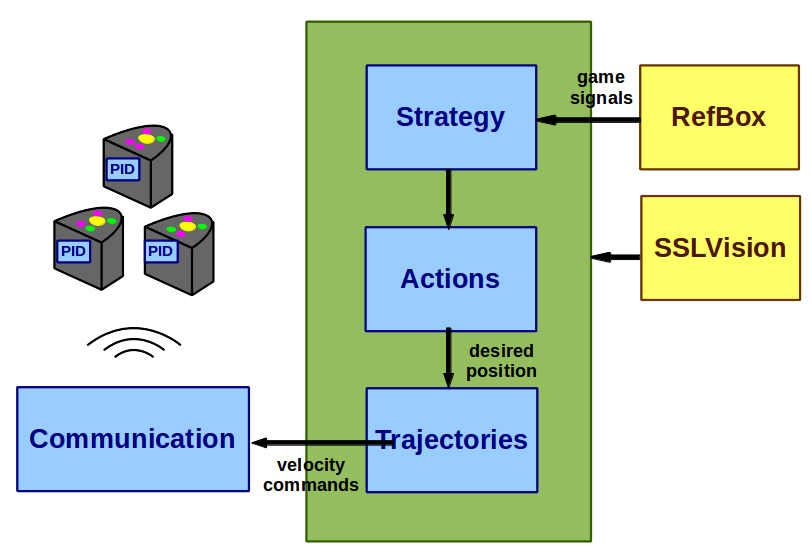
\includegraphics[width=10cm]{./pictures/eagle_knights_architecture.png}
	\caption{Eagle Knights SSL System Architecture}
	\label{fig:eagle-knights-architecture}  
\end{figure}

\TODO{Include in diagram the monitor and any other node not there yet}

We have a distributed system based on ROS (Fig.~\ref{fig:eagle-knights-architecture}) split in several nodes: Vision, Referee Box, Strategy, Action/Motion Planning, Trajectory, and Communications. A vision node is a wrapper for the SSL vision system. A referee box node is a wrapper for the SSL referee box. A strategy node defines the actions for each player  according to the state of the game, the role of the player, and the configurations of all the robots and of the ball. An action/motion planning node defines the next position for each robot according to the action it is performing and the obstacles (other robots) in the environment. A trajectory node computes the velocity commands to be sent to each robot based on their current and goal configurations. A communications node receives velocity commands for the robots and passes them through an XBee WiFi Arduino shield. A monitor node allows us to visualize the status of the robots and provide manual controls for testing.


Our robots (Fig. \ref{fig:two-ekbots}) were designed using
off-the-shelve and custom components. It has a Mojo V3 - FPGA development board for computing. We use Maxon 200142 brushless motors controlled through \emph{Afro} Electronic Speed Controllers (ESCs). For communications we use an XBee WiFi Module. We designed our own gear for speed reduction. We also designed our own dribbler and kicker. 

\TODO{Add citations for the Mojo V3 - FPGA board, for the Maxon motor, for the ESC, and for the XBee WiFi Module}

\begin{figure}[htb]
	\centering
	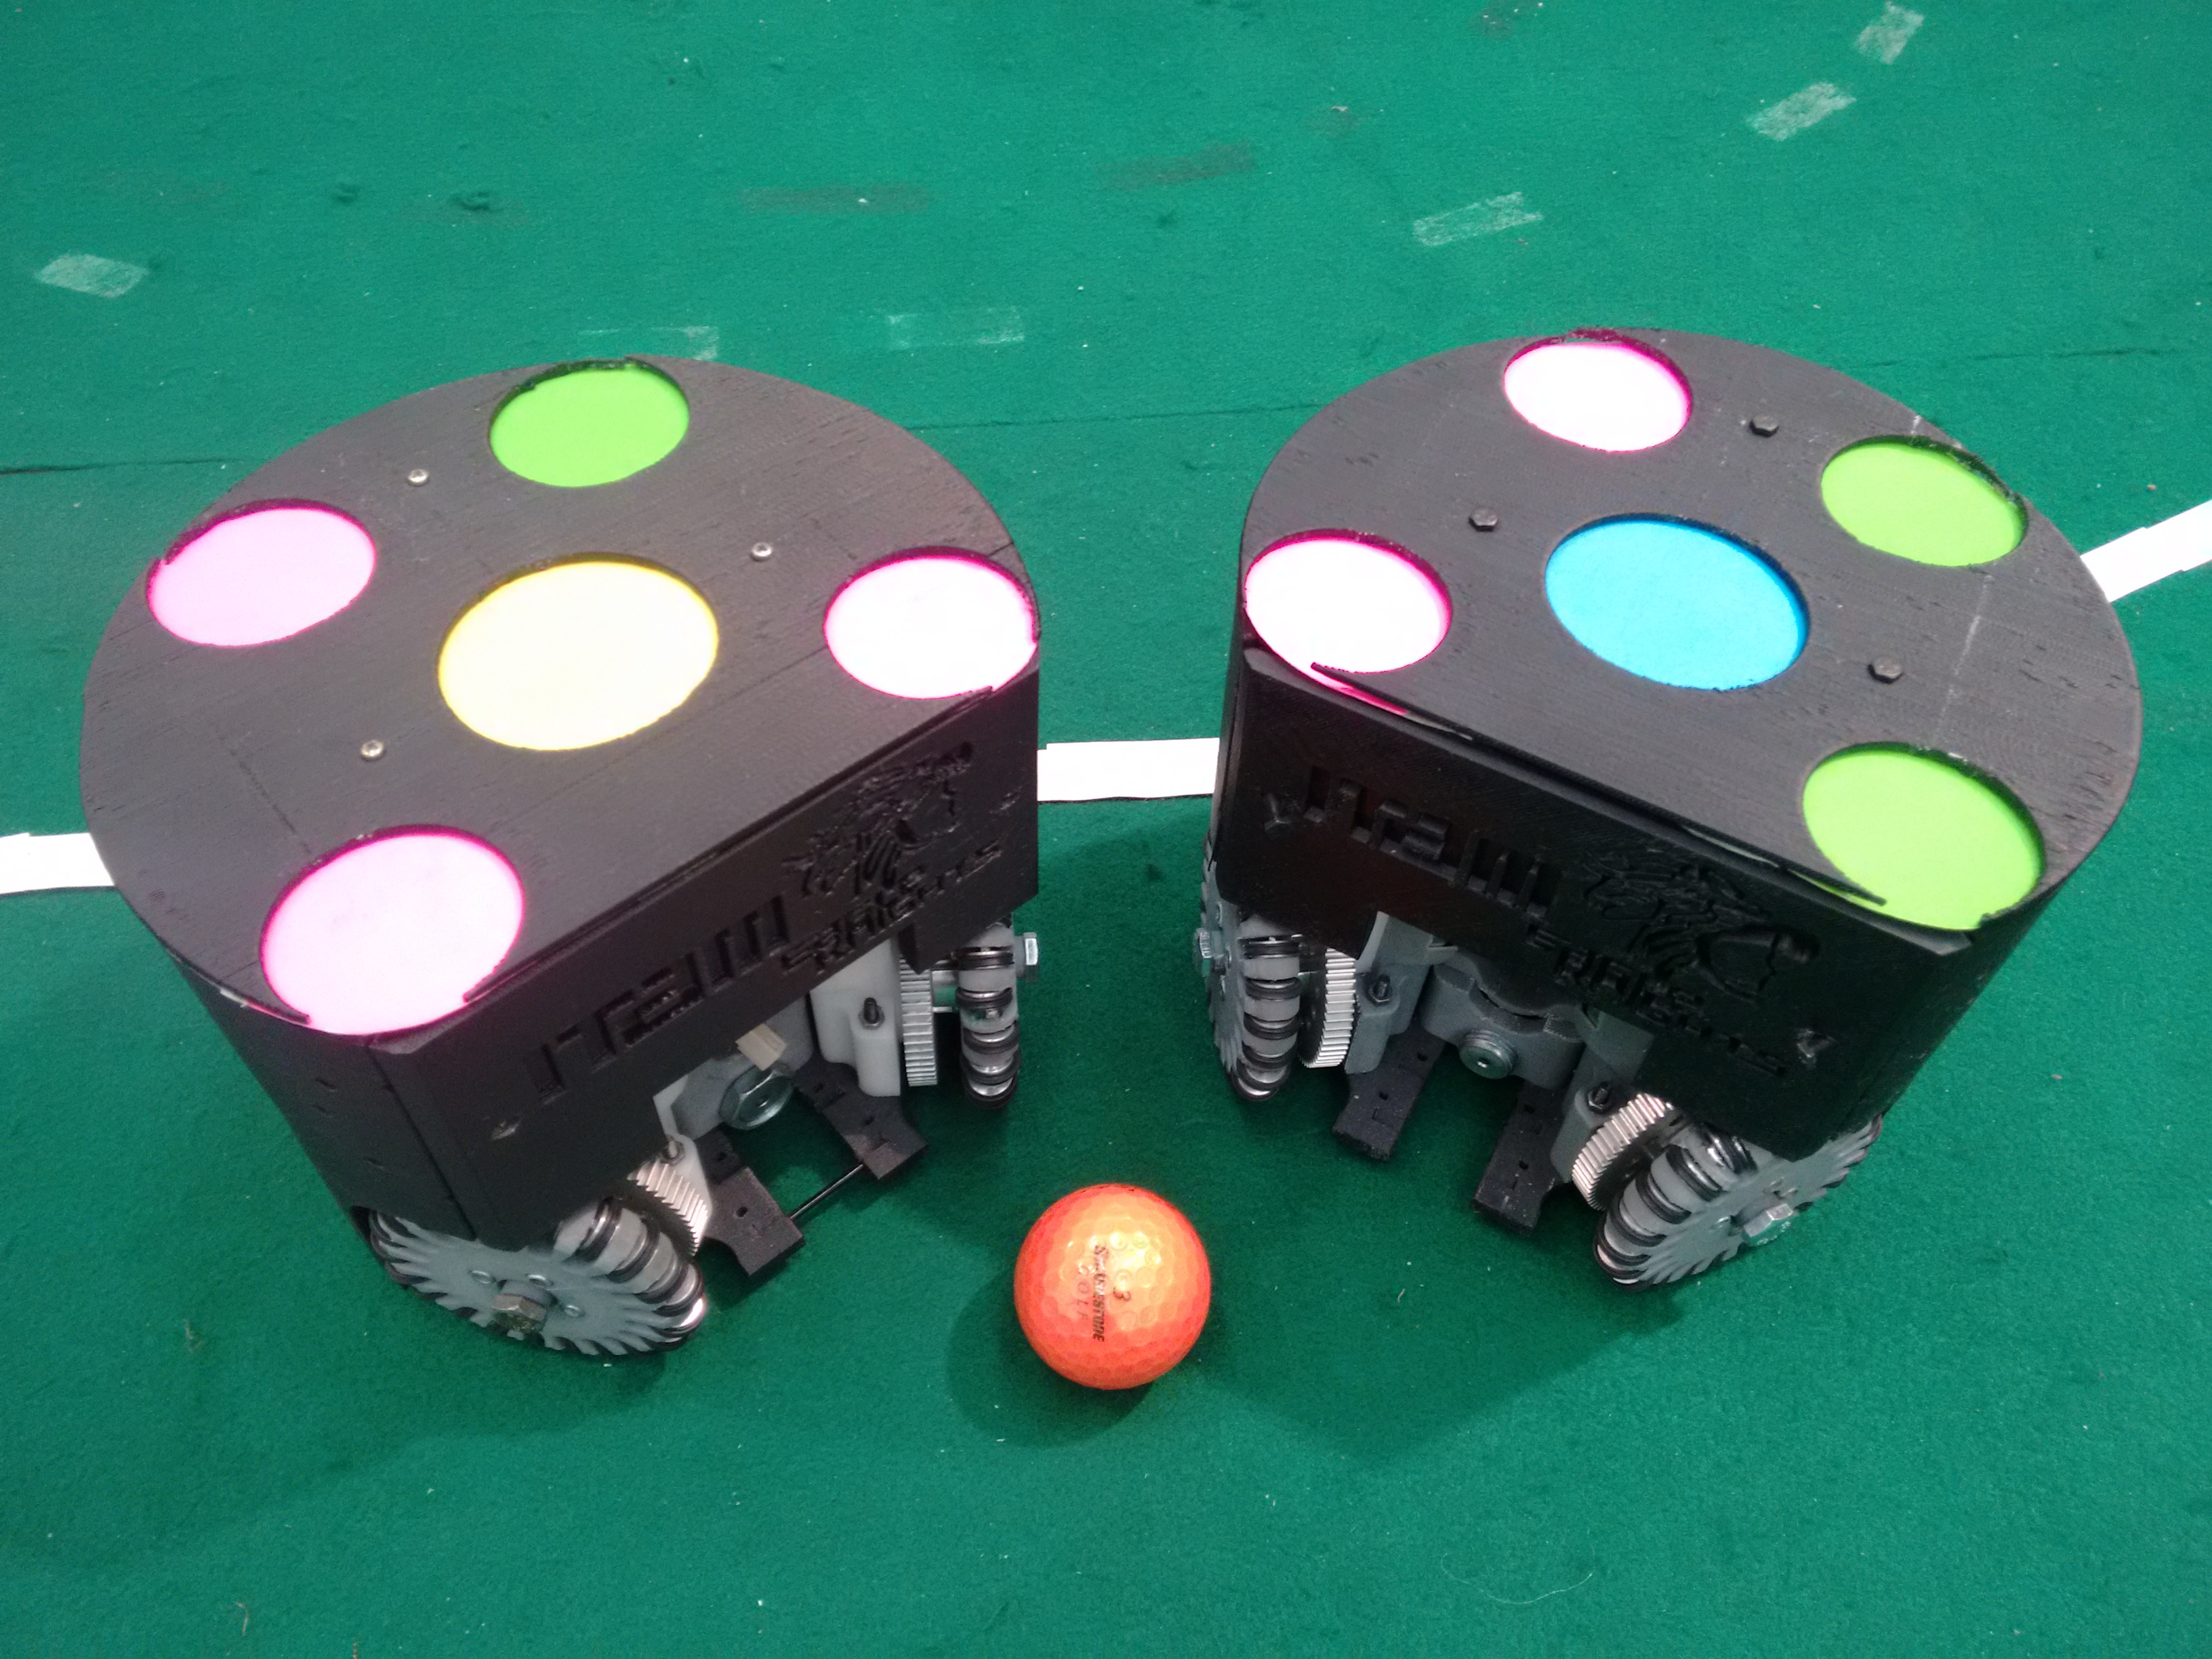
\includegraphics[width=6cm]{./pictures/two_ekbots.jpg}
	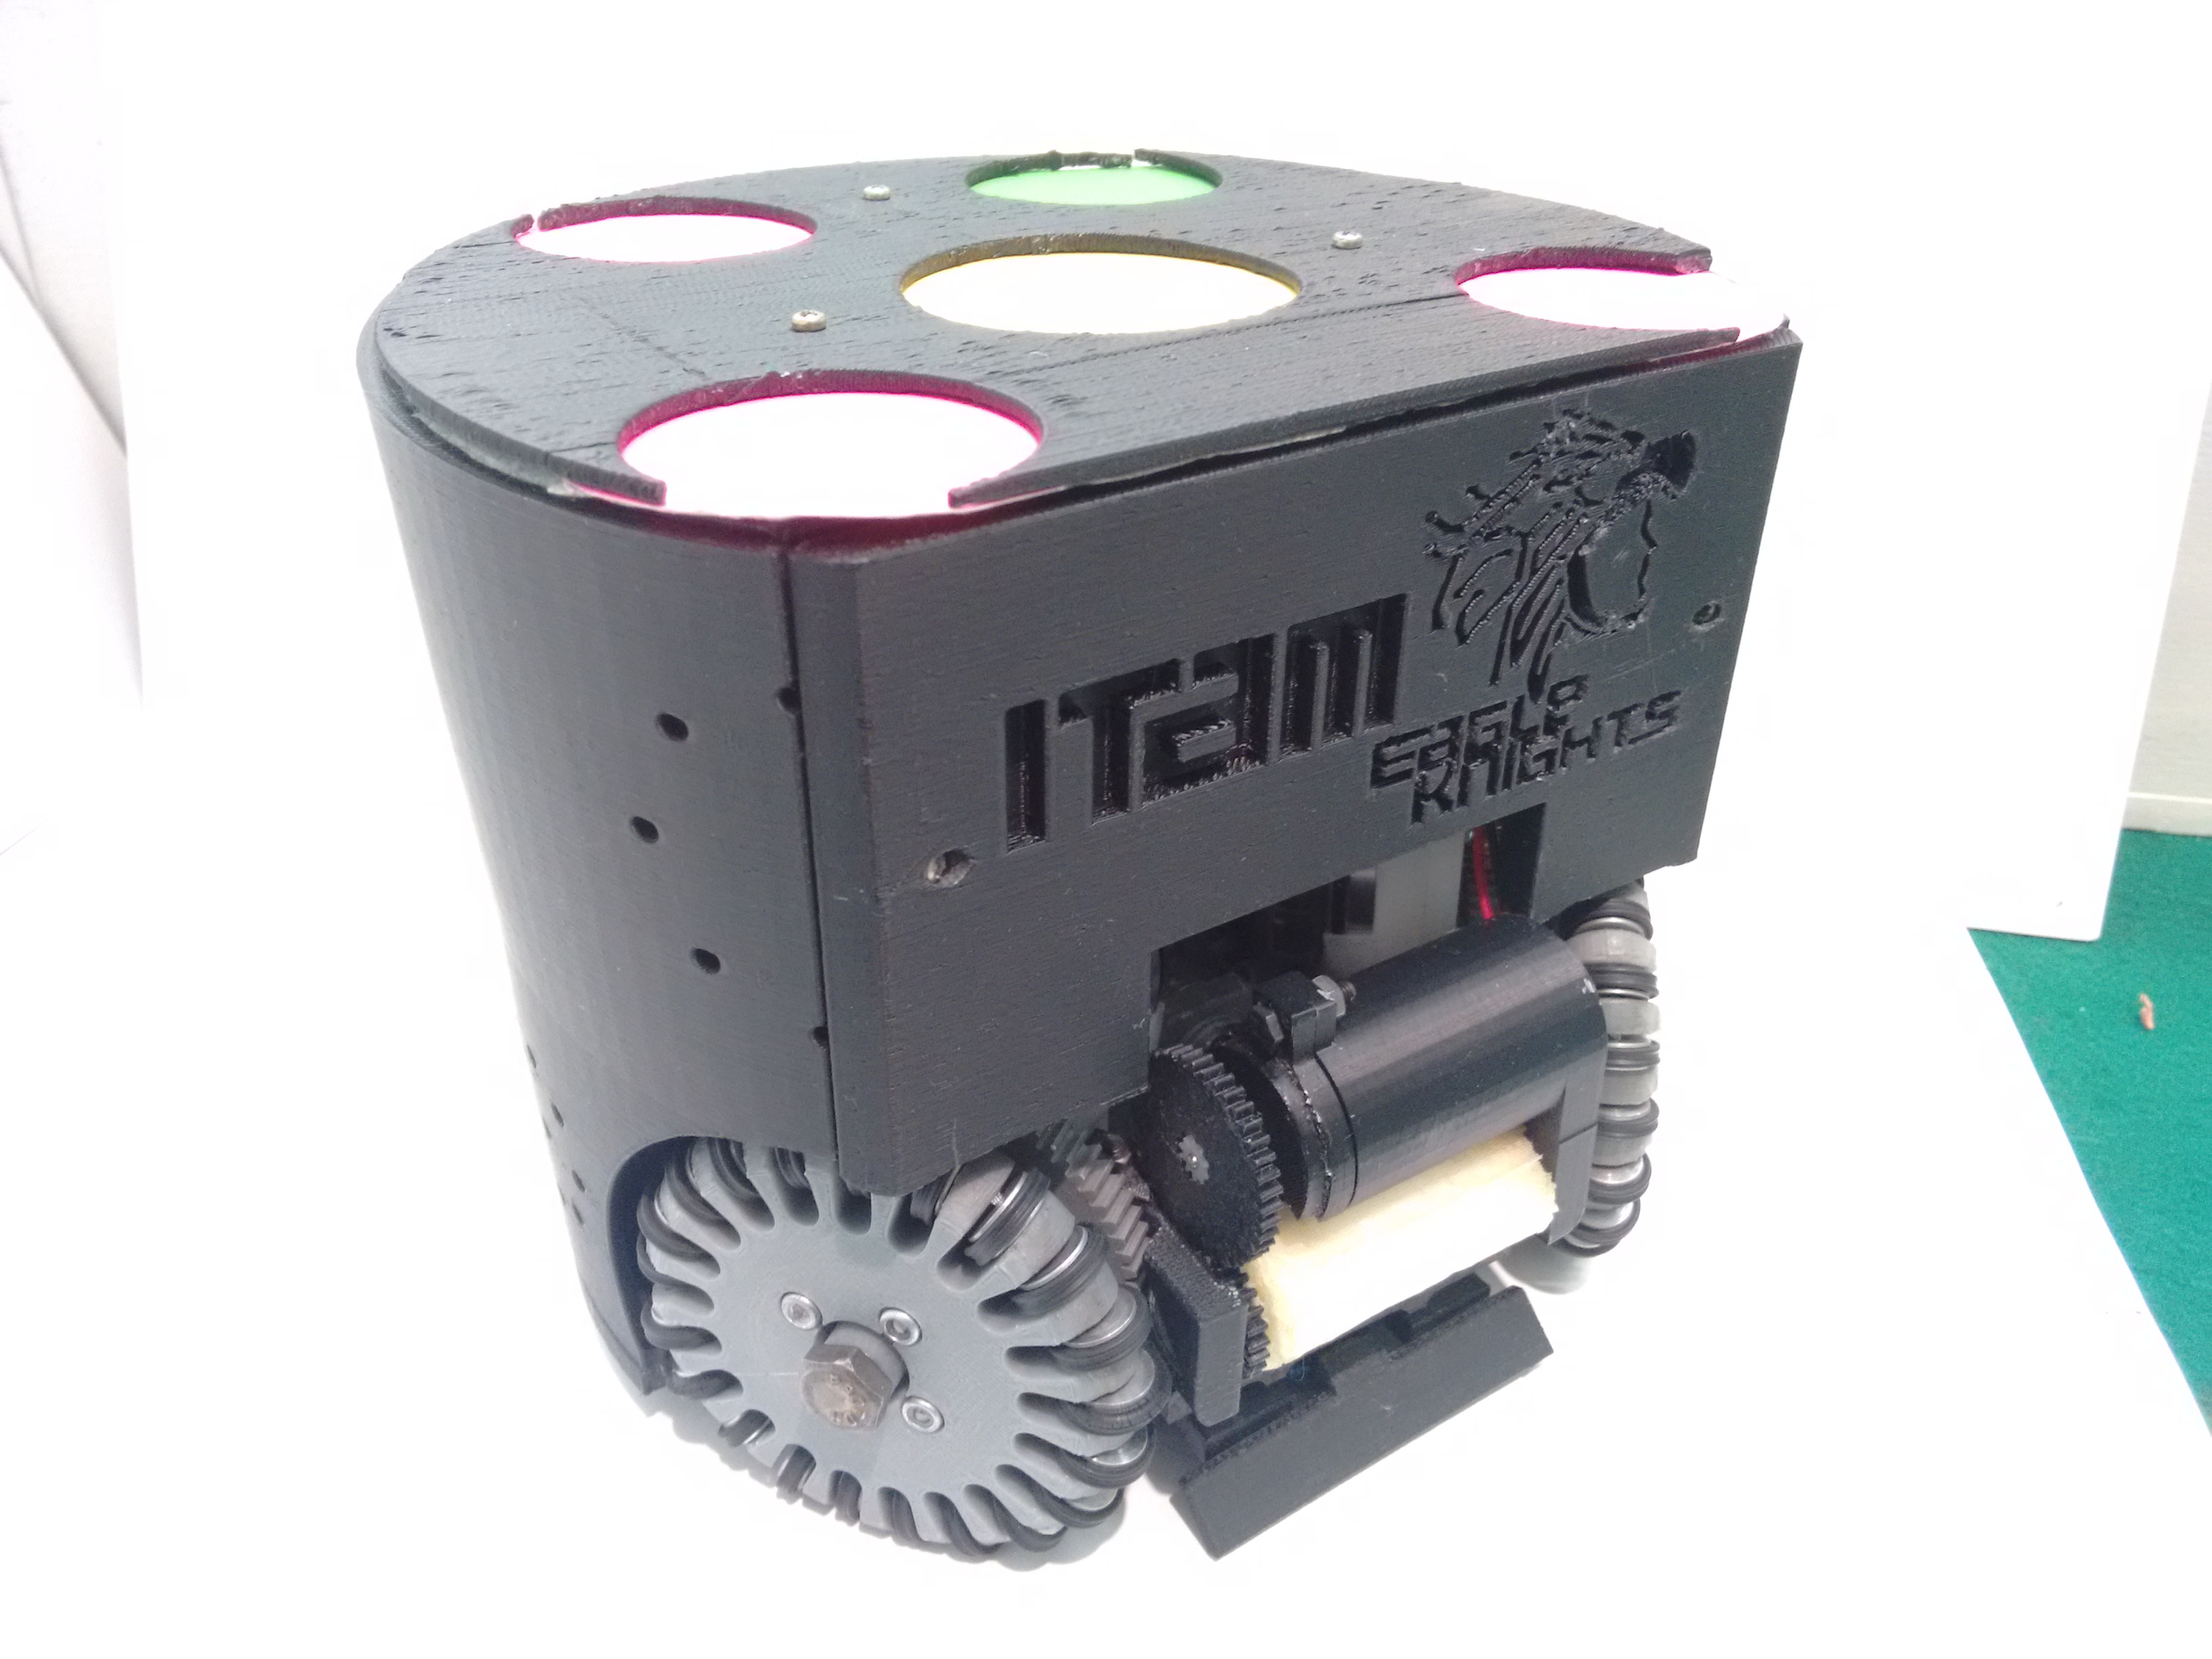
\includegraphics[width=6cm]{./pictures/ekbot_front.jpg}
	\caption{Eagle Knights SSL Robots}
	\label{fig:two-ekbots}  
\end{figure}


\section{ROS nodes}

We use the Robot Operating System (ROS) as the backbone of our system. It provides a framework to develop modular and distributed computation that has allowed us to produce compact modules that are easy to test and maintain. In ROS, we develop nodes that can communicate with each other through topics. Each node outputs information useful for other nodes through messages published to the appropriate topic. A node that needs a piece of information subscribes to the corresponding topic. Also, we can replace the robot with a robot simulator that allows us to test our algorithms even without real robots. Below, we describe each ROS node in our system.

\subsection{Monitor Node}
We have developed a Monitor with a GUI to track the robots, manual control and to display useful debugging output from the robots. 

\TODO{We need to provide more information about the Monitor and its capabilities, with one example screenshot}
%\TODO{FUTURE: EKBots simulator}
%\TODO{FUTURE: User interface for setup}


\subsection{Referee Box Node}
Our referee box node is a wrapper for the SSL referee box that communicates the state of the game as decided by
the human referee. These messages are converted into ROS topics that are used by the role node, the action node, and the trajectory node.


\subsection{Vision Node}
Our vision node is a wrapper for the SSL Shared Vision System. The Shared Vision System \cite{zlbwv-sslvtsvsftrcssl-RoboCup-2009} digitally processes the video signals from the cameras mounted on top of the field. Its main tasks are to:
\begin{description}
	\item[Capture video] in real time from cameras mounted on top of the field.
	\item[Recognize] the colored patterns specified by the rules of the robots and ball. These patterns distinguish each robot and its team (yellow or blue) through 50-mm circular patches arranged in a unique way as defined in the rules of the SSL \cite{robocup-ssl-rules}. The ball is a standard orange golf ball.
	\item[Adapt] to different lighting conditions through color calibration.
	\item[Localize] the position and orientation of robots of both teams and the position of the ball.
\end{description}

The vision node produces a ROS topic per robot and another one for the ball at a rate of 30 Hz. These topics use the Pose2D type of message from the ROS geometry\_msgs library. 


\subsection{Strategy Node}
A strategy node defines the actions for each player according to the state of the game, the role of the player, and the configurations of all the robots and of the ball. We currently support goalkeeper and forward roles with very basic strategies. The goalkeeper is always blocking the ball within the goal area. The forward follows the ball until it is close to it, and shoots towards the opposite goal.

\subsection{Action/Motion Planning Node}
An action/motion planning node defines the next position for each robot according to the action it is performing. Although several actions consist only of one move, some of them may include several distinct moves that are encoded as a state machine. At any given time, the action node produces a next position for the robot according to the active state machine. The actions that can be currently performed are: block ball, follow ball, and shoot ball. These are the action primitives:

\begin{description}
	\item[block ball] the robot moves to a point on the straight line between the robot and the ball depending on its role. If it is a goalie, it will move within the goal area, while if it is a defense, it will move outside the goal area.
	\item[follow ball] the robot moves to a point on the straight line between the robot and the ball within a small distance of the ball.
	\item[shoot ball] if the robot is far from the ball, it will move closer to the ball. If it is close to the ball, it will behind the ball on the straight line between the ball and the opposite team's goal. If it is already behind the ball, it will shoot the ball.
\end{description}

We also perform motion planning for avoiding other robots. We discretize the field into cells and we build an adjacency graph in which we only consider cells with no intersection to other robots. Then, we use the Dikjstra algorithm to find the closest path fromt the cell where the robot is located to the cell where the goal lies. Then, the path is published as the sequence of cell centers found with Dikjstra.
\TODO{provide details on parameters of graph (e.g, cell size), cite Dikjstra}

 
\subsection{Trajectory Node}
A trajectory node receives the current and goal configuration for each robot and computes the velocity command to be sent to them. This node takes in consideration the dynamic limitations of the robot to define a maximum acceleration and speed. 

In each iteration, the path provided by the Action/Motion Planning node is used as an attractor for the robot as follows. First, we compute the closest point $c_p$ on the path from the robot. Next, we compute an attractor $a$ as the point on the path and ahead of the robot that is closest to a circle centered at $c_p$ with radius $r$. This attractor is defined as the current goal for the robot that is used to compute the velocity profile to send to the robot.

\TODO{maybe a picture}

\subsection{Communications Node}
A communications node receives velocity commands for the robots and passes them through a WiFi connection.




\section{Robots}

Figure~\ref{fig:one_ekbot_inside} shows some of the internal parts of our robots.

\begin{figure}[htb]
	\centering
	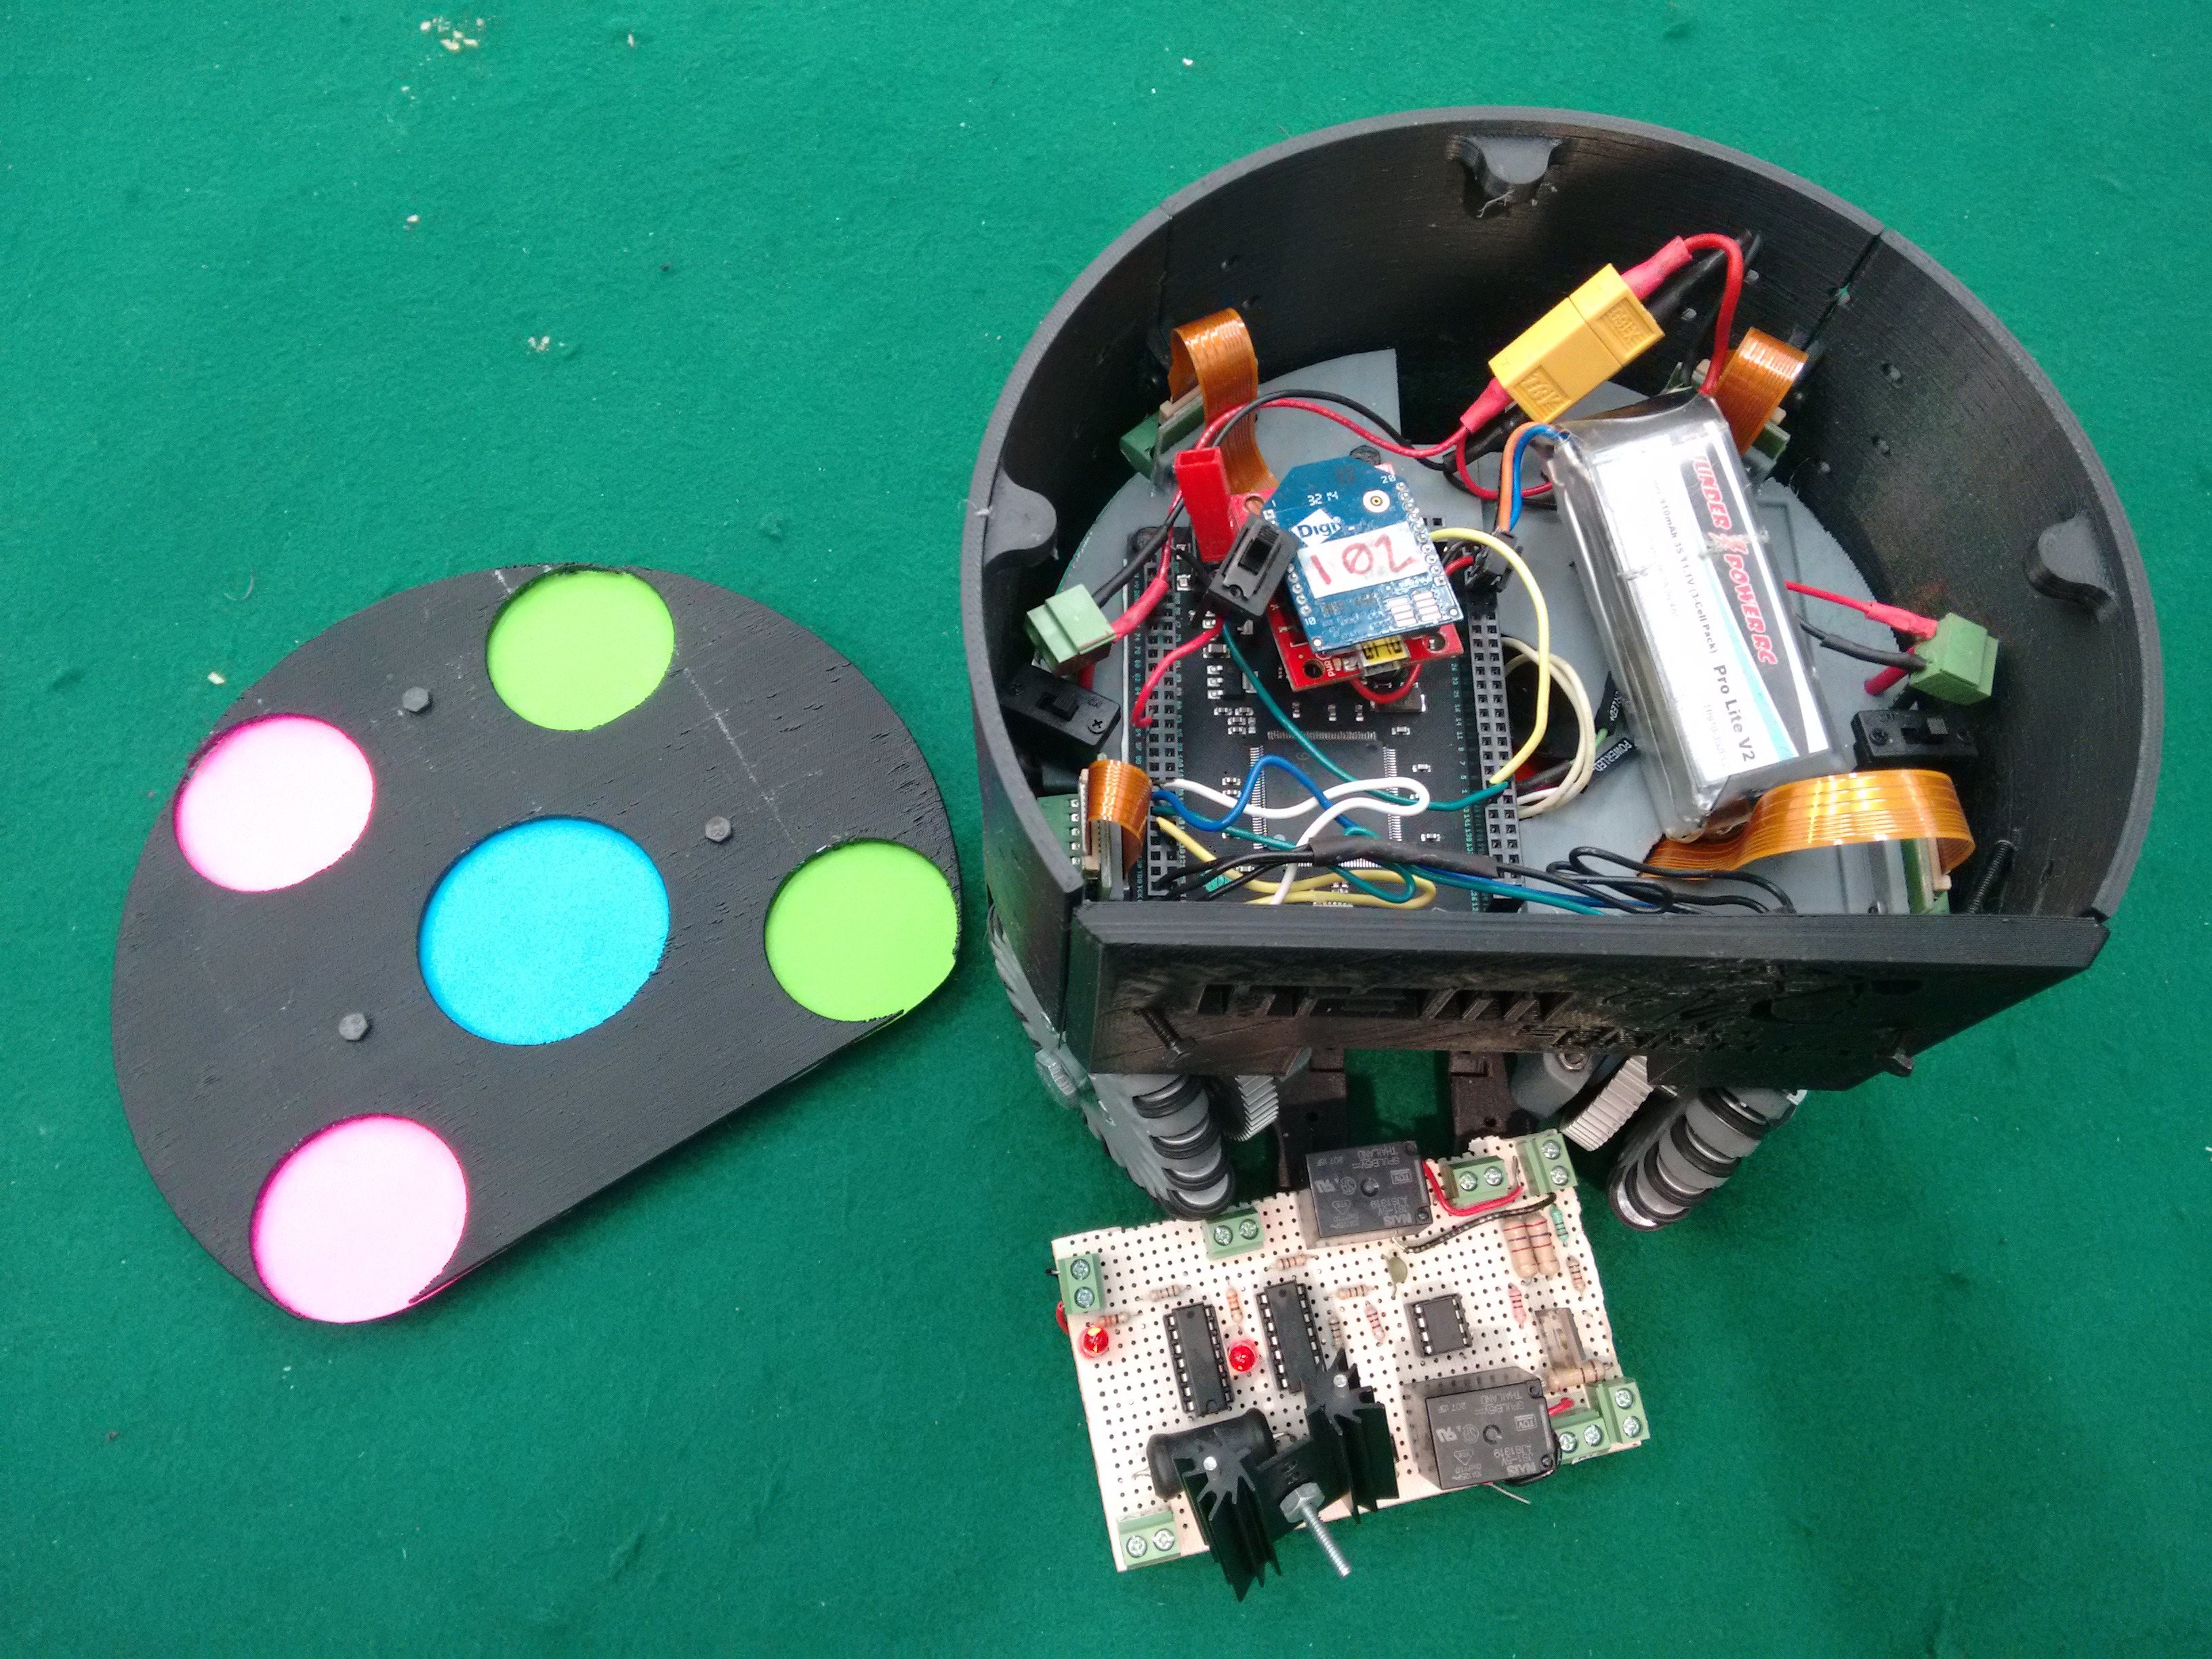
\includegraphics[width=6cm]{./pictures/one_ekbot_inside.jpg}
	\caption{Some internal parts of one of our robots}
	\label{fig:one_ekbot_inside}  
\end{figure}


\subsection{Robot Controller}
The computer on each robot performs the kinematic computations to
determine the desired speed for each motor. Also, it implements a PI
algorithm for each motor given the desired speed and the measured
speed. The later is computed through a sequential circuit that processes
the signals from the Hall sensors on the motors. 
\TODO{Summary of the kinematic model of the robot and the PID control laws} 


\subsection{Omni-Directional Drive Micro-controller}
We use the Mojo V3-FPGA development board as our on-board computing system. Since it has an ARV ATMega32 micro-controller and a Spartan 6 FPGA, we can distribute computation in the robot itself. The micro-controller transforms the desired Cartesian speeds into motor speeds. Here we implemented a mapping from robot velocities (linear and angular) to motor velocities that are fed into a controller for each motor velocity. The micro-controller also handles a PI control algorithm for each motor. Simultaneously, the FPGA handles the actual control of each motor and reads the actual motor speeds to adjust the duty cycle of the PWM signals for each motor. The WiFi communication is handled by the FPGA. 


\subsection{Actuators}
Our robots have Maxon 200142 motors with no-load speed of 4370 rpm. We have designed our own gear train with a reduction ratio of 3.5. We use a \textit{Afro} ESC for driving the motors. This allows our robots to move up to 3 m/s. Our kicker uses a low resistance solenoid.



\subsection{Kicker Control System}
Our kicker uses a push type solenoid. We have one 7.4V/ 700mA and two 11.1/900mA batteries. Since this amount of power is not enough to achieve minimum performance with the solenoid, we store energy through a voltage multiplier and discharge it when solenoid is activated. Activation happens when two conditions meet: a kicking signal is activated by the software, and an infrared sensor system in the bottom of the robot senses that the robot has the ball. 

\section{Research timeline for RoboCup 2017}
Since our last competition in RoboCup 2012, we continued with hardware improvements and we started our software from scratch. The current status of our system is that our robots can move in basic ways. We will be working in the following projects in order to get the system fully working by RoboCup 2017:

\begin{description}
	\item[Vision Node] We will complement our SSL Vision node with Kalman Filters to estimate future states of the ball and opposite robots.
	\item[Strategy Node] We currently only have a basic playing strategy. We will develop strategies for many more game situations than what we already have.
	\item[Action/Motion Planning Node] We will work intensely in having a good set of abilities for our robots.
	\item[Trajectory Node] Currently, our trajectories go at constant speed. We will try other approaches that handle better acceleration limits.
	\item[Robots] We currently have only two robots. We plan to finish putting together from four to six more.
\end{description}

\section{Some results}
Here we describe some results we have obtained with our motor controllers.
\TODO{Include the plots for motor performance and, if possible, for robot performance}

\section{Conclusions}

Here we described our robotic soccer team in order to participate in RoboCup 2017. Our current capabilities are basic, however we plan to have a team able to play by the time of the competition. Also, we have a long-term plan with the goal of having a competitive team within two years.

\TODO{Write something about performance}


\section{Acknowledgements}
This work is supported by the Asociación Mexicana de Cultura, A.C. and the Instituto Tecnológico Autónomo de México.

\bibliographystyle{unsrt}
\bibliography{robocup,robotics}


\end{document}
